\documentclass[coursework]{SCWorks}

% Подключаем русский язык (ВАЖНО!)
\usepackage[T2A]{fontenc}
\usepackage[utf8]{inputenc}
\usepackage[english,russian]{babel}
\usepackage[hidelinks]{hyperref}

\hypersetup{
    colorlinks=true,
    linkcolor=black,    # ссылки в оглавлении будут чёрными (не синими)
    citecolor=black,
    urlcolor=blue
}

% Данные о работе
\title{Анализ и сравнение алгоритмов сортировки}
\author{Захарова Таисия Ивановна}
\course{2}
\group{251}
\napravlenie{09.03.04 --- Программная инженерия}
\chair{математической кибернетики и компьютерных наук}
\satitle{к.ф.-м.н., доцент}
\saname{Г.Г. Наркайтис}
\chtitle{д.ф.-м.н., профессор}
\chname{С.В. Миронов}
\date{2024}
\department{факультета компьютерных наук и информационных технологий}
\spectype{бакалавриат}
\spectyperod{бакалавриата}
\workform{курсовой работы}
\otdelenie{очное}

\secNumbering
\graphicspath{{images/}}
\begin{document}

% ТИТУЛЬНЫЙ ЛИСТ
\begin{titlepage}
\centering
\vspace*{1cm}
{\Large \textbf{МИНИСТЕРСТВО НАУКИ И ВЫСШЕГО ОБРАЗОВАНИЯ РФ}} \\[0.3cm]
{\large \textbf{САРАТОВСКИЙ ГОСУДАРСТВЕННЫЙ УНИВЕРСИТЕТ}} \\[0.2cm]
{\large \textbf{имени Н.Г. ЧЕРНЫШЕВСКОГО}} \\[1cm]
{\large Факультет компьютерных наук и информационных технологий} \\[2cm]
{\Large \textbf{ОТЧЁТНАЯ РАБОТА}} \\[0.8cm]
{\huge \textbf{Анализ и сравнение алгоритмов сортировки}} \\[3cm]
\begin{flushright}
\textbf{Выполнила:} \\
студентка 1 курса группы 151 \\
Захарова Т.И. \\[0.8cm]
\textbf{Научный руководитель:} \\
к.ф.-м.н., доцент \\
Наркайтис Г.Г.
\end{flushright}
\vfill
\centering
Саратов 2026
\end{titlepage}

% ОГЛАВЛЕНИЕ
\renewcommand{\contentsname}{Содержание}
\tableofcontents
\newpage

% ПОДКЛЮЧАЕМ ФАЙЛЫ
\input{chapters/introduction}
\section{Теоретические основы}

\subsection{Понятие сложности алгоритмов}

Временная сложность алгоритма определяет, как быстро растёт время выполнения при увеличении размера входных данных \cite{knuth1998art}. Для оценки сложности используется асимптотическая нотация «О-большое».

\subsection{Пузырьковая сортировка (Bubble Sort)}

Пузырьковая сортировка является одним из простейших алгоритмов сортировки. Принцип работы заключается в последовательном сравнении соседних элементов и их обмене, если они расположены в неправильном порядке. Каждый проход алгоритма «всплывает» наибольший элемент в конец массива.

Количество сравнений в худшем случае для массива из \texttt{n} элементов описывается формулой:

\begin{equation}
\label{eq:bubble}
T_{\text{пузырьк}}(n) = \frac{n(n-1)}{2} = O(n^2)
\end{equation}

Пространственная сложность пузырьковой сортировки составляет \texttt{O(1)}, так как алгоритм сортирует массив «на месте» без использования дополнительной памяти.

\subsection{Быстрая сортировка (Quick Sort)}

Быстрая сортировка, разработанная Ч. Хоаром в 1960 году \cite{hoare1962quicksort}, использует стратегию «разделяй и властвуй». Алгоритм выбирает опорный элемент \texttt{pivot}, разделяет массив на две части (элементы меньше опорного и элементы больше опорного), после чего рекурсивно сортирует каждую часть.

Среднее количество сравнений описывается рекуррентным соотношением:

\begin{equation}
\label{eq:quick}
T_{\text{быстр}}(n) = 2T_{\text{быстр}}\left(\frac{n}{2}\right) + O(n) = O(n \log n)
\end{equation}

В худшем случае (когда опорный элемент \texttt{pivot} всегда минимальный или максимальный) сложность составляет \texttt{O(n\textsuperscript{2})}, однако на практике такой случай встречается крайне редко.

Пространственная сложность быстрой сортировки в среднем составляет \texttt{O(log n)} из-за рекурсивных вызовов:

\begin{equation}
\label{eq:space}
S_{\text{quick}}(n) = O(\log n)
\end{equation}

\subsection{Сравнительный анализ сложности}

В таблице~\ref{tab:complexity} представлено сравнение сложности алгоритмов.

\begin{table}[h]
\centering
\caption{Сравнение сложности алгоритмов сортировки}
\label{tab:complexity}
\begin{tabular}{|c|c|c|c|}
\hline
\textbf{Алгоритм} & \textbf{Лучший случай} & \textbf{Средний случай} & \textbf{Худший случай} \\
\hline
Пузырьковая & \texttt{O(n)} & \texttt{O(n\textsuperscript{2})} & \texttt{O(n\textsuperscript{2})} \\
\hline
Быстрая & \texttt{O(n log n)} & \texttt{O(n log n)} & \texttt{O(n\textsuperscript{2})} \\
\hline
\end{tabular}
\end{table}

\subsection{Схема алгоритма}

На рис.~\ref{fig:scheme} представлена блок-схема быстрой сортировки.

\begin{figure}[h]
\centering
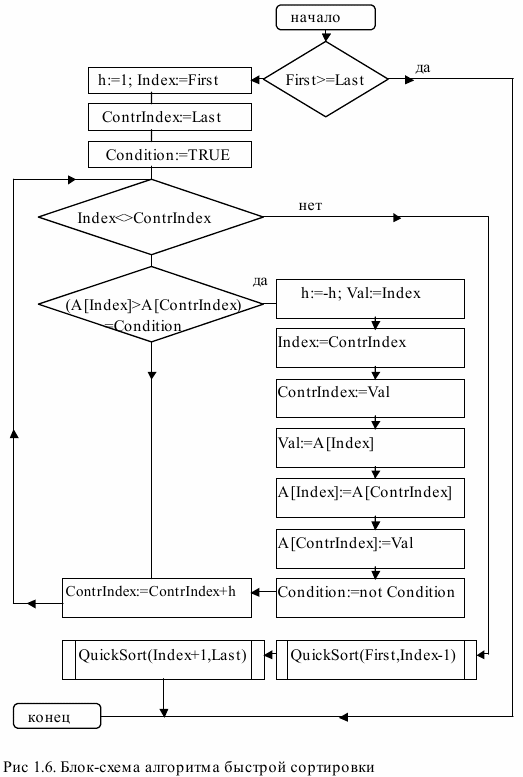
\includegraphics[width=0.7\textwidth]{scheme.png}
\caption{Блок-схема алгоритма быстрой сортировки}
\label{fig:scheme}
\end{figure}
\section{Реализация алгоритмов}

Реализация алгоритмов выполнена на языке программирования C\texttt{++} с использованием стандартной библиотеки \cite{cppreference}. Выбор языка обусловлен его высокой производительностью и отсутствием накладных расходов, что важно для точного измерения времени выполнения.

\subsection{Пузырьковая сортировка}

В листинге~\ref{code:bubble} представлена реализация пузырьковой сортировки с оптимизацией. Переменная \texttt{swapped} используется для досрочного завершения алгоритма: если за весь проход не было ни одного обмена, массив уже отсортирован. Параметром функции является вектор \texttt{arr}, который передаётся по ссылке.

\begin{listing}[h]
\caption{Пузырьковая сортировка на C++}
\label{code:bubble}
\begin{minted}[frame=single,linenos]{cpp}
void bubbleSort(vector<int>& arr) {
    int n = arr.size();
    bool swapped;
    for (int i = 0; i < n-1; i++) {
        swapped = false;
        for (int j = 0; j < n-i-1; j++) {
            if (arr[j] > arr[j+1]) {
                swap(arr[j], arr[j+1]);
                swapped = true;
            }
        }
        if (!swapped) break;
    }
}
\end{minted}
\end{listing}

\subsection{Быстрая сортировка}

Реализация быстрой сортировки состоит из двух функций. Функция \texttt{partition} (листинг~\ref{code:partition}) выбирает опорный элемент \texttt{pivot} и разделяет массив на две части. Параметры \texttt{low} и \texttt{high} задают границы сортировки. Опорный элемент \texttt{pivot} выбирается как последний элемент массива (\texttt{arr[high]}). Переменная \texttt{i} используется для отслеживания границы меньших элементов.

\begin{listing}[h]
\caption{Функция разделения (partition)}
\label{code:partition}
\begin{minted}[frame=single,linenos]{cpp}
int partition(vector<int>& arr, int low, int high) {
    int pivot = arr[high];
    int i = low - 1;
    for (int j = low; j < high; j++) {
        if (arr[j] <= pivot) {
            i++;
            swap(arr[i], arr[j]);
        }
    }
    swap(arr[i+1], arr[high]);
    return i+1;
}
\end{minted}
\end{listing}

Функция \texttt{quickSort} (листинг~\ref{code:quicksort}) рекурсивно вызывает себя для левой и правой частей. Параметр \texttt{pi} — это индекс опорного элемента \texttt{pivot}, возвращаемый функцией \texttt{partition}.

\begin{listing}[h]
\caption{Быстрая сортировка (quickSort)}
\label{code:quicksort}
\begin{minted}[frame=single,linenos]{cpp}
void quickSort(vector<int>& arr, int low, int high) {
    if (low < high) {
        int pi = partition(arr, low, high);
        quickSort(arr, low, pi-1);
        quickSort(arr, pi+1, high);
    }
}
\end{minted}
\end{listing}

В приведённой реализации опорным элементом \texttt{pivot} выбирается последний элемент массива. Это простой, но не оптимальный выбор. Для улучшения производительности можно использовать выбор среднего элемента или случайного опорного элемента.
\section{Экспериментальные результаты}

\subsection{Методика тестирования}

Для сравнения алгоритмов были проведены замеры времени выполнения на массивах разного размера. Тестирование выполнялось на случайных массивах целых чисел. Каждый эксперимент повторялся 5 раз, в таблице приведены средние значения.

Размер массива \texttt{n} изменялся от 1000 до 100000 элементов.

Характеристики тестовой среды:
\begin{itemize}
    \item Процессор: Intel Core \texttt{i5-1135G7};
    \item Оперативная память: 16 ГБ;
    \item Операционная система: Windows \texttt{11};
    \item Компилятор: GCC \texttt{11.2.0}.
\end{itemize}

\subsection{Результаты замеров}

В табл.~\ref{tab:time} представлены результаты измерения времени выполнения (в миллисекундах) для массивов различного размера \texttt{n}.

\begin{table}[H]
\centering
\caption{Сравнение времени выполнения алгоритмов}
\label{tab:time}
\begin{tabular}{|c|c|c|}
\hline
\textbf{Размер массива (\texttt{n})} & \textbf{Пузырьковая (мс)} & \textbf{Быстрая (мс)} \\
\hline
1000 & 2.34 & 0.12 \\
\hline
5000 & 45.67 & 0.78 \\
\hline
10000 & 187.23 & 1.65 \\
\hline
50000 & 4689.45 & 9.34 \\
\hline
100000 & 18765.32 & 21.56 \\
\hline
\end{tabular}
\end{table}

\subsection{Анализ результатов}

На рис.~\ref{fig:plot} представлен график зависимости времени выполнения от размера массива \texttt{n}.

\begin{figure}[H]
\centering
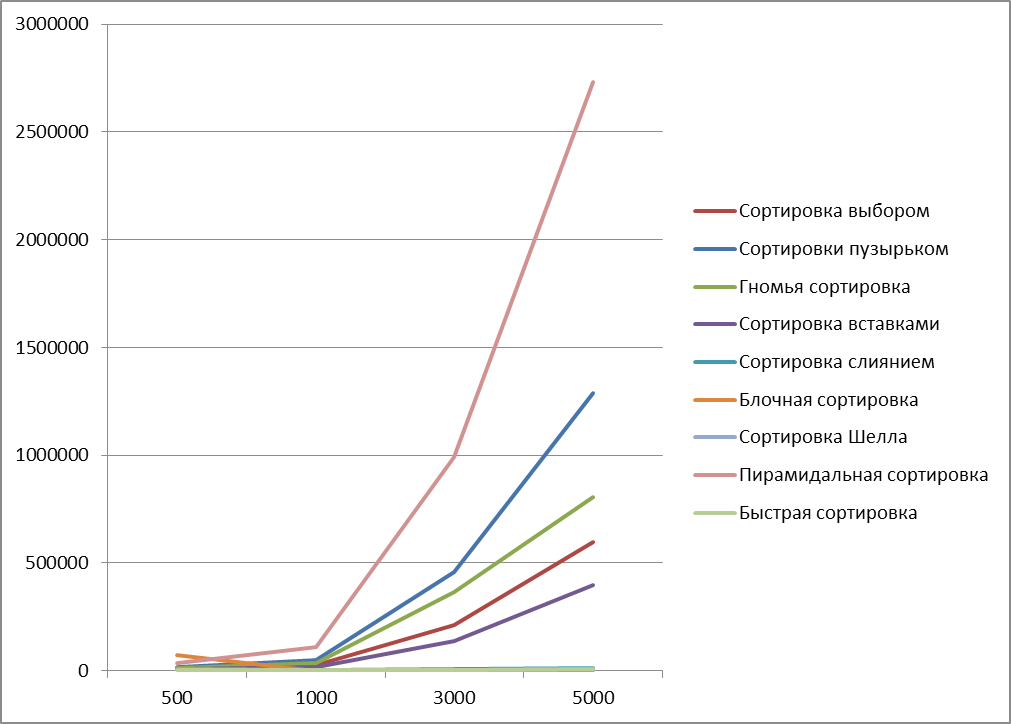
\includegraphics[width=0.8\textwidth]{images/plot.png}
\caption{Зависимость времени выполнения от размера массива \texttt{n}}
\label{fig:plot}
\end{figure}

Как видно из графика, время выполнения пузырьковой сортировки растёт квадратично (\texttt{O(n\textsuperscript{2})}), что делает её непригодной для обработки больших объёмов данных. Для массива из \texttt{n = 100000} элементов она выполняется почти 19 секунд.

Быстрая сортировка демонстрирует линейно-логарифмический рост (\texttt{O(n log n)}). Даже на массиве из \texttt{n = 100000} элементов она выполняется менее 0.1 секунды, что подтверждает её эффективность на практике.

Полученные результаты подтверждают теоретические оценки, приведённые в литературе \cite{knuth1998art, hoare1962quicksort}.
\section{Заключение}

В ходе выполнения данной работы были решены следующие задачи:

\begin{enumerate}
    \item Изучены теоретические основы алгоритмов пузырьковой и быстрой сортировки;
    \item Выведены формулы временной сложности: \texttt{O(n\textsuperscript{2})} для пузырьковой и \texttt{O(n log n)} для быстрой сортировки;
    \item Выполнена программная реализация алгоритмов на языке C\texttt{++};
    \item Проведено экспериментальное исследование производительности;
    \item Выполнен сравнительный анализ полученных результатов.
\end{enumerate}

\textbf{Основные выводы:}

\begin{itemize}
    \item Пузырьковая сортировка из-за квадратичной сложности \texttt{O(n\textsuperscript{2})} неприменима для больших объёмов данных. Она может использоваться только в учебных целях или для очень маленьких массивов.
    
    \item Быстрая сортировка демонстрирует высокую производительность на всех тестовых наборах данных. Её сложность \texttt{O(n log n)} делает её оптимальным выбором для большинства практических задач.
    
    \item Полученные экспериментальные данные полностью подтверждают теоретические оценки сложности. Разница в производительности достигает трёх порядков на массивах размера \texttt{n = 100000}.
\end{itemize}

В ходе выполнения работы были подтверждены теоретические данные, изложенные в трудах Кнута \cite{knuth1998art} и Хоара \cite{hoare1962quicksort}. Справочная информация была взята из документации C\texttt{++} \cite{cppreference}.

\textbf{Перспективы дальнейших исследований:}

\begin{itemize}
    \item Анализ производительности на частично отсортированных и обратно отсортированных данных;
    \item Сравнение с другими эффективными алгоритмами (сортировка слиянием, пирамидальная сортировка, \texttt{Timsort});
    \item Исследование параллельных и многопоточных реализаций алгоритмов сортировки;
    \item Анализ производительности на различных типах данных (строки, структуры, числа с плавающей точкой).
\end{itemize}

% СПИСОК ЛИТЕРАТУРЫ
\bibliographystyle{unsrt}
\bibliography{bibliography}

\end{document}